%-------------------------------------------------------------------------------
% Theorie
%-------------------------------------------------------------------------------
\section{Theoretischer und empirischer Hintergrund}
Leistung ist je nach Kontext unterschiedlich definiert. Im Rechnungswesen werden unter Leistung etwa die im Produktionsprozess entstandenen Güter und Dienstleistungen und der damit verbundenen Wertezuwachs für das Unternehmen oder den Markt verstanden \cite{woeltje2010abc}. Im Zivilrecht hingegen ist Leistung als Handlung oder Unterlassung definiert, zu der der Schuldner aufgrund eines Schuldverhältnisses verpflichtet ist (§ 241 I BGB). Zwar unterscheiden sich die einzelnen Definitionen im Detail teilweise deutlich, dennoch haben alle Leistungsbegriffe gemein, dass damit eine (wie auch immer geartete) zu Ergebnissen führende Anstrengung bezeichnet wird. Diese Anstrengung geht in der Regel von einem menschlichen Individuum aus, das sie, in Form von körperlicher oder geistiger Arbeit, erbringt. Die Gründe, warum Menschen Arbeit leisten, sind vielfältig und komplex. Neben monetären Anreizen gibt es unterschiedliche nichtmonetäre Beweggründe, die Menschen dazu motivieren, freiwillig und von sich aus eine Arbeit zu verrichten. Dazu gehören Anerkennung, sozialer Status, Spaß und Selbstverwirklichung \cite{shujaat}. Eine weitere Möglichkeit zur Erhöhung der Leistung durch gesteigerte Motivation ist Gamification. 

\subsection{Definition Gamification}
Mit dem Begriff Gamification wird ein vergleichsweise junges Forschungs- und Wirtschaftsgebiet beschrieben. Erste dokumentierte Aufzeichnungen des Begriffs stammen aus dem Jahr 2008 \cite{huotari_defining_2012, deterding_game_2011}. Konkrete Verwendung fand der Begriff jedoch erst im Jahr 2010, wobei er zunehmend in Industrie und Wirtschaft eine Rolle spielt \cite{huotari_defining_2012}. Konzerne, wie Fourthsquare, haben zu diesem Zeitpunkt damit begonnen, Spielmechaniken in ihre Dienste zu integrieren, um die Nutzerinteraktion zu erhöhen \cite{deterding_game_2011}.

Im Laufe der Zeit sind unterschiedliche Definitionen für Gamification entstanden. Die geläufigste stammt von \citeauthorwithyear{deterding_game_2011}. Die Autoren verstehen unter Gamification den Einsatz von Spieldesignelementen in einem spielfremden Kontext \cite{deterding_game_2011}. Gemeint ist damit die Integration dessen, was ein Spiel ausmacht (Abzeichen, Level, Erfahrungspunkte, Trophäen), in eine spielfremde Tätigkeit, etwa die Lehre, die Arbeit oder den Haushalt. Zwei praktische Beispiele aus der Realität sind Duolingo und Reddit. So kann der Nutzer auf der Lernplattform Duolingo, die der interaktiven Vermittlung von Sprachkenntnissen dient, als Belohnung für den Abschluss bisheriger Lektionen ständig neue Lektionen freischalten. Bei dem Social-News-Aggregator Reddit hingegen ist ein ausgeklügeltes Punktesystem integriert. Nutzer können auf der Plattform durch das regelmäßige Posten qualitativ hochwertiger Beiträge 'Karmapunkte' sammeln. Gleichzeitig ist es für jeden Nutzer möglich, eben diese Beiträge mit einem 'Down-Vote' oder einem 'Up-Vote' zu bewerten. Ziel ist es, dass sich Nutzer freiwillig engagieren, um ihr Ansehen in der Community zu steigern.

\citeauthorwithyear{deterding_game_2011} unterscheiden grundsätzlich zwischen den Begriffen \textit{Game} und \textit{Play}. Mit \textit{Game} ist dabei das konkrete Spiel gemeint, das sich durch definierte Ziele und Regeln auszeichnet, während als \textit{Play} das freie, regellose und improvisierte Spielen bezeichnet wird. Der Begriff \textit{Play} ist damit weiter gefasst und schließt das \textit{Game} ein. So kann der Begriff \textit{Play} beispielsweise mit dem übermütigen, ausgelassenen Umherspringen von Kindern illustriert werden. \textit{Gaming} hingegen beschreibt ein ziel- und regelgebundenes Spielen, wie etwa ein Fußballspiel. Die Art des Spielens muss dabei nicht zwangsläufig Spaß bringen oder der reinen Unterhaltung dienen. Für den professionellen Fußballspieler trägt das Spiel vielmehr zu seiner Existenzgrundlage bei und wird nicht zur Unterhaltung betrieben. An diesem Beispiel zeigt sich auch, dass Gamification nicht auf digitale Medien beschränkt ist.  Spiele und Spielelemente sind vielmehr transmediale Kategorien ohne klare Grenzen zwischen digital und nicht-digital \cite{deterding_game_2011}.

Aus dieser Unterscheidung lässt sich jene zwischen \textit{Gamefulness} und \textit{Playfulness} ableiten. Beide Begriffe bezeichnen die Erlebnis- und Verhaltenseigenschaften der jeweiligen Kategorie. Obwohl Gamification und \textit{Gamefulness} in der Regel zusammen fallen, da sich beide Begriffe auf die Strategie der Verwendung von Spielelementen für das Erzeugen spielerischer Erfahrungen beziehen, unterscheiden sich die Begriffe hinsichtlich ihrer intensionalen Eigenschaften: Als Gamification wird die Designstrategie hinter der Verwendung von Spielmechaniken bezeichnet, während \textit{Gamefulness} das eigentliche Ziel des spielerischen Designs bezeichnet \cite{deterding_game_2011}. Das Konzept des \textit{Playful Designs} beschreibt dagegen den Versuch, verschiedene Tätigkeiten spielerischer und damit angenehmer zu gestalten. Unter diese Tätigkeiten fallen sämtliche Aktivitäten, die Freunde und Spaß vermitteln (z. B. Lesen), weshalb es sich, nicht zwangsläufig um Spiele oder Spielelemente handeln muss.


\subsubsection{Serious Games}
Während unter Gamification die Integration \textbf{einzelner} Spieldesignelemente in einen spielfremden Kontext zu verstehen ist, werden als Serious Games vollwertige Spiele bezeichnet, die nicht ausschließlich der Unterhaltung dienen \cite[S. 17]{michael_serious_2005}. Dabei handelt es sich um eigenständige Spiele (\textit{whole game}) und nicht bloß um die Integration individueller Spielelemente (\textit{game parts}) \cite{deterding_game_2011}. Diese Art von Spiel wird häufig mit der Absicht entworfen, dem Spieler einen Lerninhalt spielerisch zu vermitteln. Dabei ist es nicht entscheidend, ob der Spieler das Spiel als Lerninhalt betrachtet oder als reine Unterhaltung \cite[S.3]{bopp_serious_2009}. Analog dazu lassen sich Spielzeuge und \textit{Playful Design} voneinander unterscheiden. Spielzeuge (\textit{toys}) sind vollwertige Gegenstände, die spielend genutzt werden. Als \textit{Playful Design} wird bezeichnet dagegen der Versuch/ die Intention bezeichnet, beliebige Tätigkeiten spielerischer zu gestalten.

\begin{figure}[htp]
    \centering
    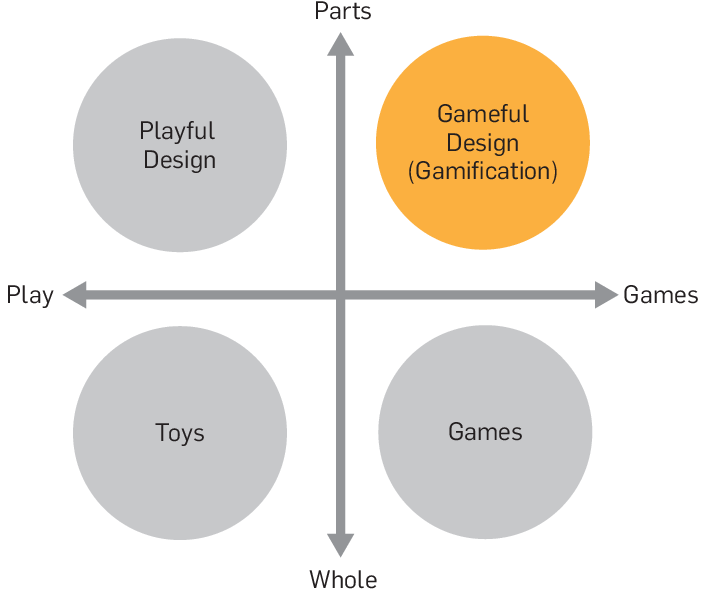
\includegraphics{img/detering_gamificatrion_pic.png}
    \caption{Abgrenzung von Gamification, Serious Games und Playful Design (Deterding  et  al.,2011)}
    \label{fig:deterding}
\end{figure}

Serious Games lassen sich grob in die Kategorien Educational  Games, 
Corporate  Games,  Health  Games,  Persuasive  Games,  Music  Games  sowie  Virtual  Worlds  und 
Mobile Learning Games unterteilen \cite[S.4]{bopp_serious_2009}.
Für die vorliegende Arbeit ist lediglich die Kategorie der Educational  Games relevant.
Bei dieser Art von Serious Games geht es um den pädagogischen Einsatz von Videospielen.
Charakteristisch für Educational  Games ist, dass die Lernerfahrung auf ein spezifisches Ziel ausgerichtet ist \cite{nielsen_overview_2006, bopp_serious_2009}.
Typischerweise besteht ein derartiges Ziel in der Vermittlung bestimmter Fähigkeiten, wie Algebra, Rechtschreibung und weiteren Grundfertigkeiten.
Derartige Spiele fallen auch unter den Oberbegriff Edutainment \cite{nielsen_overview_2006} und bieten den Spielern befriedigende Aufgaben, die zu der Entwicklung von neuen Fähigkeiten und Strategien führen können \cite{stapleton_serious_2004}.
\citeauthorwithyear{vlachopoulos_effect_2017} bestätigen die umfassende empirische Evidenz in Bezug auf kognitive Lernergebnisse einschließlich Wissenserwerb, konzeptuelle Anwendung und Inhaltsverständnis.

Obwohl es eine Vielzahl von Educational Games gibt, müssen nicht zwangsläufig vollwertige Spiele entworfen werden, um einen positiven Effekt in der Lehre zu erreichen. Nicht nur zu Serious Games, sondern auch zum Einsatz von Spielmechaniken in der Bildung wird derzeit umfassend geforscht \cite{ibanez_gamification_2014,landers_enhancing_2017}. Da der Lernerfolg wesentlich von der Motivation, dem Interesse und dem Engagement der Lernenden bedingt ist \cite{astin_student_1984}, sind Spielmechaniken ein vielversprechendes Mittel, um die Leistung der Lernenden zu erhöhen.
Dieser Bereich zählt neben Gesundheit und Fitness zu den empirisch am besten untersuchten Anwendungsgebieten in der Gamificationforschung \cite{koivisto_rise_2019}.
So konnten positive Effekte auf Motivation und Leistung in der Praxis nachgewiesen werden \cite{ibanez_gamification_2014,hamzah_influence_2015,strmecki_gamification_2015}. Weniger Ergebnisse, jedoch tendenziell vielversprechende Ansätze finden sich im Kontext der Programmierung, die thematisch zahlreiche Überschneidungen hinsichtlich der Bedienung der Kommandozeile aufweist. So konnten \citeauthorwithyear{layth_khaleel_empirical_2019} eine Verbesserung der Lernleistung im Kontext von Programmieraufgaben feststellen. Zu ähnlichen Ergebnissen kommen \citeauthorwithyear{ortiz_gamification_2017}. Anzumerken ist jedoch, dass letztere zwar eine Verbesserung des Engagements feststellen konnten, allerdings keine Auswirkungen auf die Motivation ersichtlich war.



% Kurzer Text zu unterschiedlichen Spiellementen
\subsection{Spielelemente}\label{gamelelements}
Ebenso wie der Begriff Gamification sind auch die Spielelemente in unterschiedlicher Weise definiert. Ein naiver Ansatz könnte sein, Spielelemente als Reihe von spielspezifischen Bausteinen und Merkmalen zu definieren. Es stellt sich jedoch die Frage, was spielspezifisch tatsächlich bedeutet. Bei einer strengen Auslegung dieser Definition würde sich z.B. nur eine sehr kleine Menge von Spielelementen ergeben. Avatare, Abzeichen oder Ranglisten sind in der Gamification häufig verwendete Spielelemente. Gleichwohl findet sich für jedes genannte Spielelement ein spielfremdes Gegenbeispiel. So werden Avatare auch auf Jobbörsen verwendet (LinkedIn), Abzeichen als Verdienstauszeichnung für besondere Leistungen verliehen (Bundesverdienstkreuz) und Ranglisten auf Produktvergleichsportalen verwendet (Stiftung Warentest). Eine sehr liberale Auslegung der Definition würde wiederum Elemente einschließen, die nicht als Spielelemente zu betrachten sind. Als Beispiele seien hier Waffen und die Darstellung Gewalt genannt - wobei beides in vielen Spielen durchaus vorkommt.

\citeauthorwithyear{deterding_game_2011} schlagen daher vor, Gamifizierung auf die Beschreibung von Elementen zu beschränken, die für Spiele charakteristisch sind - Elemente, die in den meisten (aber nicht notwendigerweise allen) Spielen zu finden sind, die leicht mit Spielen in Verbindung gebracht werden können und eine bedeutende Rolle im Spiel einnehmen. Die Autoren weisen explizit darauf hin, dass es sich um eine heuristische Definition handelt, die viel Raum für Diskussionen darüber bietet, was "charakteristisch" für Spiele ist. \citeauthorwithyear{Reeves2009Total} haben in diesem Zusammenhang zehn Spielelemente identifiziert, die 'gelungene' Spiele ausmachen:

\begin{enumerate}
  \item die Möglichkeit der Selbstdarstellung (Avatar)
  \item das Vorhandensein einer räumlichen Spielwelt (3D Welt)
  \item ein Narrativ (Eine Geschichte, die das Spiel leitet)
  \item direktes Feedback
  \item Punktesysteme, Ranglisten und Level (Reputation)
  \item Marktplätze und Ökonomien
  \item Wettbewerbsregeln 
  \item Teams
  \item gegenseitiger Austausch und Kommunikation unter den Spielern
  \item Zeitdruck
\end{enumerate}

Die beiden für diese Arbeit relevanten Spielelemente sind Abzeichen und Fortschrittsbalken. Abzeichen stellen eine Anerkennung für erbrachte Leistung dar und können damit zu den 'gelungenen' Spielelementen (Reputation) gezählt werden. Die Fortschrittsanzeige erlaubt Rückschlüsse auf die Gesamtdauer des Experiments und gibt zudem direktes Feedback über den eigenen Fortschritt. Beide Designelemente lassen sich außerdem vergleichsweise einfach in eine Terminalemulation integrieren, da jedes Spielelement in sich abgeschlossen ist und keine Abhängigkeiten von anderen Designelementen besteht. Dadurch, dass sowohl Abzeichen als auch Fortschrittsanzeige eigenständig funktionieren sollten, ist zudem eine individuelle Bewertung des jeweiligen Spielelements möglich. Dies ermöglicht die Beurteilung der tatsächlichen Wirksamkeit und der Effektivität der einzelnen Spielelemente. Eine solche Einzelfallbetrachtung ist in der Wissenschaft nicht zwangsläufig gegeben. Tatsächlich weisen \citeauthorwithyear{mazarakis2018gamification} in ihrer Analyse darauf hin, dass es nahezu unmöglich ist, den tatsächlichen Beitrag einzelner Spielelemente in Bezug auf die Motivationssteigerung zu messen, da sie häufig kombiniert eingesetzt werden. Aus diesem Grund ist es sinnvoll, einzelne Spielelemente individuell zu untersuchen.


%-------------------------------------------------------------------------------
% Abzeichen
%-------------------------------------------------------------------------------
\subsubsection{Spielelement Abzeichen}\label{badge}
Das Abzeichen ist eines der prominentesten Spielelemente und dürfte aus dem Alltag bekannt sein. Konzerne die Abzeichen in ihren Produkten einsetzen sind zum Beispiel TripAdvisor, Google, Starbucks oder GitHub. Konkret handelt es sich dabei um digitale, visuelle Artefakte, die dem Nutzer für die Erfüllung definierter Aufgaben verliehen werden \cite{antin_badges_2011}. \citeauthorwithyear{antin_badges_2011} unterteilen Abzeichen anhand ihrer sozialpsychologische Funktion in fünf Kategorien: Zielsetzung (Goal setting), Anweisung (Instruction), Reputation (Reputation),
Status/Bestätigung (Status / Affirmation) und Gruppenidentifizierung (Group Identification). 


\paragraph{Zielsetzung}
Abzeichen fordern den Nutzer dazu heraus, ein definiertes Ziel zu erreichen. Individuen streben selbst dann nach dem Erreichen bestimmter Ziele oder Meilensteine, wenn sie selbst keinerlei physische Gegenleistung erfahren. Die durch ein Abzeichen dargestellten Ziele sind allerdings nicht immer explizit, etwa weil die notwendigen Aktivitäten subjektiv oder unpräzise definiert sind. Aus diesem Grund ist es zentral, den Nutzer durch regelmäßiges Feedback auf seinen aktuellen Fortschritt hinzuweisen. 

\paragraph{Anweisung}
Abzeichen können richtungweisend wirken. Sie geben Hinweise darauf, welche Arten von Aktivitäten innerhalb eines Systems möglich sind. Diese Funktion ist nützlich, um neue Benutzer in eine bestimmte Richtung zu lenken, aber auch um bestehenden Nutzern neue Wege zu offenbaren. Dabei ist es nicht notwendig, dass Nutzer die Abzeichen tatsächlich erreichen, denn das bloße Betrachten der verfügbaren Abzeichen gibt dem Nutzer Aufschluss über wertgeschätzte Aktivitäten.

\paragraph{Reputation}
Abzeichen bilden die Grundlage für die Reputationsbewertungen einzelner Nutzer. Durch die Kapselung von Interessen, Fachwissen und vergangener Interaktionen helfen Abzeichen bei der Beurteilung der Reputation. So geben einsehbare Abzeichen einen Einblick in nutzerspezifische Interessen, bieten einen Überblick über Fähigkeiten und Fachwissen und dienen der Einschätzung der Vertrauenswürdigkeit und der Zuverlässigkeit eines Nutzers. Zugleich enthalten sie Hinweise auf bereits erbrachte Leistungen.

\paragraph{Status/Bestätigung}
Abzeichen wirken als eine Art Statussymbol. Sie verdeutlichen die eigene Leistung und bisherige Errungenschaften ohne explizite Prahlerei.
Die Macht der Statusbelohnungen ergibt sich insbesondere aus der Erwartung, dass andere positiv auf jemanden reagieren, der aufgrund außerordentlicher Aktivitäten entsprechende Abzeichen erhalten hat. Abzeichen dienen auch als persönliche Bestätigung, da sie an vergangene Errungenschaften erinnern. Sie markieren Meilensteine und sind ein Beweis für vergangene Erfolge. Sie wirken damit auf eine ähnliche Art und Weise wie klassische Trophäen oder Medaillen.

\paragraph{Gruppenidentifizierung}
Über die Abzeichen wird eine Reihe von gemeinsamen Aktivitäten kommuniziert, die eine Gruppe von Benutzern anhand der kollektiven Erfahrung verbindet. Das Erlangen von Abzeichen kann ein Gefühl der Solidarität vermitteln und die positive Gruppenidentifikation durch die Wahrnehmung der Ähnlichkeit zwischen einem Individuum und der Gruppe erhöhen.\\

Es gibt zahlreiche wissenschaftliche Arbeiten, in denen die Wirksamkeit von Abzeichen analysieren. Unterschiedliche Arbeit kommen dabei zu teilweise gegensätzlichen Ergebnissen. So konnten \citeauthorwithyear{ortiz_gamification_2017} durch den Einsatz von Abzeichen zwar eine statistisch signifikante Verbesserung des Engagements der Lernenden feststellen. Allerdings war keine Verbesserung der Leistung und der intrinsischen Motivation erkennbar. Gleichermaßen stellten \citeauthorwithyear{dominguez_gamifying_2013} in einem pädagogischen Kontext fest, dass Abzeichen zwar einen positiven Einfluss auf praktische Aufgaben haben, aber potentiell negativ auf schriftliche Abgaben wirken. \citeauthorwithyear{toda_dark_2018} weißt sogar explizit auf die Gefahr einer Reduzierung der Leistung, unerwünschter Seiteneffekte und potentiellem Motivationsverlust hin. Dieses Risiko gilt es den zahlreichen positiven Effekten gegenüber zu stellen. Zu nennen ist hier insbesondere das gesteigerte Engagement, welches von unterschiedlichen Autoren beobachtet werden konnte \cite{ortiz_gamification_2017, dominguez_gamifying_2013, hamari_badges_2017, hamzah_influence_2015}. Damit bleiben Abzeichen ein überaus vielversprechendes Spielelement. 


%-------------------------------------------------------------------------------
% Fortschrittsbalken
%-------------------------------------------------------------------------------
\subsubsection{Spielelement Fortschrittsbalken}\label{progressbar}
Das Spielelement Fortschrittsbalken ist ebenfalls ein etabliertes visuelles Spielelement.
Dabei handelt es sich um ein visuelles Anzeigeelement, durch das der aktuellen Fortschritt eines Auftrags in Form eines Balkens repräsentiert wird. Dabei können selbst einfachste Fortschrittsanzeigen positiv auf die Motivation der Nutzer wirken \cite{mazarakis2018gamification}. Ein klassisches Beispiel ist etwa die Darstellung des Fortschritts einer Installation oder eines Ladevorgangs. Im Wesentlichen lassen sich Fortschrittsanzeigen in zwei Kategorien einteilen: Zum einen gibt es die bestimmte Anzeige, die den absoluten Fortschritt eines Vorgangs anzeigt. Anhand der Anzeige kann somit Aufschluss auf die verbleibende Restdauer des Vorgangs gewonnen werden. Häufig wird bei bestimmte Anzeigen zusätzlich eine Prozentangabe verwendet. Auf der anderen Seite existieren unbestimmte Fortschrittsanzeigen, die keinerlei Rückschluss auf den aktuellen Fortschritt erlauben. Dies kann beispielsweise durch einen Teilbalken realisiert werden, der sich fortwährend von links nach rechts bewegt. Fortschrittsanzeigen finden sich sehr häufig in digitalen Systemen, wie etwa Computerprogrammen, oder in Umfragen. Im letzten Fall werden entsprechenden Anzeigen in der Regel verwendet, um eine höhere Abschlussquote zu erreichen. Diese Annahme lässt sich jedoch anhand empirischer Untersuchungen nicht bestätigen \cite{Heerwegh}. So verzeichneten Umfragen mit Fortschrittsbalken geringere Abschlussquoten als Umfragen ohne Fortschrittsindikatoren \cite{liu_examining_2017}. Dennoch ist auch die Fortschrittsanzeige ein vielversprechendes Spielelement. Allerdings liegen zu diesem Aspekt deutlich  weniger Forschungsergebnisse vor als zu anderen Spielelementen \cite{koivisto_rise_2019}. Zum anderen gibt es durchaus positive Ergebnisse: \citeauthorwithyear{olsson_visualisation_2016} kommen in ihrer Arbeit zu dem Ergebnis, dass ein Fortschrittsbalken eine geeignete Maßnahme ist, um den Überblick der Kursteilnehmer in Online-Umgebungen zu verbessern. Gleichzeitig weisen die Autoren auf einen möglichen positiven Einfluss von Abzeichen auf die Motivation der Teilnehmer hin. Dies kann durch das Gefühl der Vollendung erklärt werden, welches wiederum ein Gefühl der Zufriedenheit vermittelt \cite{ryan_deci_2000}.

\subsection{Motivationstheorie}
Es existieren unterschiedlichste Modelle, die die Wirkung von Gamification erklären. Ein weit verbreiteter Ansatz ist die Selbstbestimmungstheorie nach \citeauthorwithyear{ryan2017self}. Diese wird sehr häufig verwendet, um die Wirkung von Gamification zu erklären\cite{rapp2019strengthening}.

\subsubsection{Selbstbestimmungstheorie}
Gemäß der Selbstbestimmungstheorie (\textit{Self Determination Theory}, kurz SDT) nach \citeauthorwithyear{ryan2017self} wird davon ausgegangen, dass Menschen Fleiß und Mühe in die Erbringung einer Leistung investieren, wenn drei wesentliche psychologische Grundbedürfnisse erfüllt sind: Kompetenz (\textit{Competence}), Autonomie (\textit{Autonomy}) und Zugehörigkeit (\textit{Relatedness}).

 \paragraph{Kompetenz}
 Mit Kompetenz ist im Kern das Bedürfnis gemeint, eine Aufgabe zu meistern. Dieses Bedürfnis ist erfüllt, wenn sich die Person fähig fühlt und das Gefühl hat, eine Aufgabe effektiv zu bewältigen \cite{ryan2017self}. Dies ist insbesondere dann der Fall, wenn das Individuum den Anforderungen gerecht wird und die eigenen Fähigkeiten als ausreichend wahrgenommen werden. Gleichwohl ist das Grundbedürfnis nach Kompetenz nicht erfüllt, wenn der Anspruch einer Aufgabe die eigenen Fähigkeiten übersteigt oder die ausführende Person ausschließlich negatives Feedback erhält. Geeignete Spielelemente, die das subjektiv wahrgenommene Gefühl der Kompetenz positiv beeinflussen, sind nach \citeauthorwithyear{sailer2016wirkung} Punkte, Leistungsgraphen oder Ranglisten. Durch diese Spieldesignelemente erhält der Nutzer ein positives Feedback und die die eigene Leistungsfähigkeit wird hervorgehoben.
 
 
 \paragraph{Autonomie}
 Unter Autonomie verstehen \citeauthorwithyear{ryan2017self} das Grundbedürfnis der Wahlfreiheit. Dieses Bedürfnis ist erfüllt, wenn das Individuum das Gefühl hat, sich freiwillig und ohne äußeren Zwang für bestimmte Tätigkeiten entscheiden zu können. Diese Tätigkeiten sollten den eigenen Wertvorstellungen entsprechen und als positiv wahrgenommen werden. Zusätzlich muss die Person möglichst in der Lage sein, das eigene Handeln eigenständig zu steuern, und sich selbst als Herr der eigenen Entscheidungen fühlen. Negativ wirken äußere Zwänge, unzureichende Wahlmöglichkeiten oder fehlendes Mitspracherecht. Auch dieses Bedürfnis kann durch Spielelemente zusätzlich befriedigt werden. So lässt sich beispielsweise durch Avatare das Gefühl der Wahlfreiheit erhöhen \cite{sailer2016wirkung}.
  
\paragraph{Zugehörigkeit}
Das Bedürfnis nach Zugehörigkeit und sozialer Eingebundenheit ist erfüllt, wenn sich eine Person mit anderen Personen verbunden fühlt. Diese Verbundenheit entsteht durch sozialen Kontext und durch subjektiv wahrgenommene, soziale Nähe. Fühlen sich Personen nicht in der Lage, einen Mehrwert für die Gruppe zu liefern, oder empfinden sich entsprechende Personen überhaupt nicht als Teil einer Gruppe, kann dieses Bedürfnis nicht erfüllt werden. Durch gemeinsame Teambestenlisten kann das subjektiv wahrgenommene Gefühl des konstruktiven Wettbewerbs erhöht werden \cite{sailer2016wirkung}.


Durch die hier gewählten Abzeichen und Fortschrittsbalken soll das Kompetenzbedürfnis bedient werden. Ein Fortschrittsbalken gibt Aufschluss über den eigenen Fortschritt und liefert damit Kompetenzfeedback - ähnlich wie es bei dem durch \citeauthorwithyear{sailer2016wirkung} vorgeschlagenen Punktesystem der Fall ist. Abzeichen wirken ähnlich, indem bisherigen Leistungen bestätigt werden und gleichzeitig die eigene Leistungsfähigkeit demonstriert werden kann \cite{antin_badges_2011}. Aufgrund der Tatsache, dass das Erlernen der Kommandozeile mit viel Frustration verbunden sein kann und damit potentiell negativ auf das Kompetenzbedürfnis wirkt, erscheinen die gewählten Spielelemente vielversprechend.

%-------------------------------------------------------------------------------
% HCI - Kommandozeile
%-------------------------------------------------------------------------------
\subsection{Kommandozeile}
Die Kommandozeile, auch Befehlszeile, CLI (Command Line Interface) oder Terminal genannt, stellt die einfachste Form der Mensch-Computer-Interaktion dar \cite{Kumar2005}. Ein dieses Programm werden Textzeilen als Eingabe akzeptiert, die dann kontextabhängig ausgeführt werden. Diese Aufgabe übernimmt der Befehlsinterpreter, der die über die Tastatur eingegebenen Befehle interpretiert und anschließend ausführt \cite{wissen_interpreter}. 
Dadurch ist es dem Nutzer möglich, externe Programme zu starten sowie Konfigurationsänderungen oder Manipulationen des Dateisystems vorzunehmen (Erstellen, Kopieren, Löschen von Dateien und Ordnern).

Kommandozeilen haben einen wesentlichen Vorteil gegenüber graphischen Oberflächen: Durch die Kombination unterschiedlicher Befehle und Parameter ist es möglich, komplexe Arbeitsabläufe mit minimaler Interaktion abzubilden. Für den Nutzer zeigt sich dies in einer gesteigerte Effizienz \cite{Kumar2005}. Gleichzeitig ist die Entwicklung einer Konsolenschnittstelle für den Entwickler mit deutlich weniger Aufwand verbunden als die Entwicklung einer graphischen Oberfläche. Dennoch erfordert die Bedienung der Kommandozeile das Wissen über Befehle, möglicher Befehlsparameter und der entsprechenden Syntax für den jeweiligen Interpreter. Das Erlernen des Umgangs mit der Kommandozeile ist damit vergleichbar mit dem Erlernen einer Programmiersprache. Tatsächlich gibt es für etablierte Kommandozeilen eigene Skriptsprachen, die dem programmatischen Ausführen von Befehlen dienen (Bash, DOS, ZSH, usw.). Aufgrund dieser Eigenschaften werden Kommandozeilen insbesondere im professionellen Umfeld eingesetzt. Neben dem Einsatz in der Softwareentwicklung und Systemadministration finden sich Kommandozeilen in vielen Programmen, die auch über eine graphische Oberfläche verfügen. So verfügen AutoCAD, Adobe Photoshop, SAP und die Microsoft Office-Produkte über zusätzliche Interaktionsmöglichkeiten per Kommandozeile.



%-------------------------------------------------------------------------------
% Fragestellung
%-------------------------------------------------------------------------------

\subsection{Fragestellung und Zielsetzung}
Das Erlernen des Umgangs mit der Kommandozeile gleicht in Teilen dem Erlernen einer Programmiersprache und kann anfänglich mit einem hohen Maß an Frustration verbunden sein. Daher bietet es sich an, den Lernprozess motivierender zu gestalten, um den Lernerfolg zu erhöhen. So gibt es zahlreiche und im weitesten Sinne 'gamifizierte' Konsolenanwendungen im Internet. Es handelt sich häufig um interaktive Text-Adventures. Als Beispiele können hierfür LostKingdom\footnote{Link: https://rdebath.github.io/LostKingdom/}, TheLab\footnote{Link: https://gfc.albertocongiu.com/thelab/}und Adventex\footnote{Link: https://thoster.net/adventex/} gennant werden. Die Wirksamkeit entsprechender Anwendungen wurde bisher jedoch nie empirisch untersucht. 

Im Rahmen der Arbeit werden daher die Spielelemente Abzeichen und Fortschrittsbalken in eine Webanwendung integriert, die der Vermittlung grundlegender Kommandozeilenbefehlen dient. Anschließend wird der Einfluss der Spielelemente hinsichtlich Motivation und Leistung der Benutzer untersucht. Wie in Abschnitt \ref{gamelelements} geschildert, zeigen beide Spielelemente positive Effekte auf die Lernleistung von Lernenden und sind daher vielversprechende Designelemente. Die der Arbeit zugrundeliegende Forschungsfrage lautet daher:

\begin{itemize}
    \item Welchen Einfluss haben die Spieldesignelemente Abzeichen und Fortschrittsbalken auf die Motivation und die Leistung im Kontext der Kommandozeile?
\end{itemize}

Daraus lassen sich die folgenden Hypothesen ableiten:

\begin{itemize}
\item H1: Probanden, die Abzeichen erhalten, beantworten im Mittel eine höhere Anzahl an Fragen als eine Kontrollgruppe ohne Abzeichen.
\item H2: Probanden, die eine Fortschrittsanzeige sehen, beantworten im Mittel eine höhere Anzahl an Fragen als eine Kontrollgruppe ohne Fortschrittsanzeige.
\end{itemize}

Die Ergebnisse sind für alle Personen interessant, die Berührungspunkte mit der Kommandozeile haben.
Hervorzuheben sind insbesondere Schüler und Studenten, die keinerlei bestehende Erfahrung mit einer rein textbasierten Nutzerschnittstelle haben. Die entstehende Anwendung könnte zukünftig dazu dienen, Einsteigern beim Erlernen des Umgangs mit der Kommandozeile zu unterstützen. Gleichzeitig liefert die Arbeit weitere empirische Daten hinsichtlich der Wirkung von Abzeichen und Fortschrittsanzeige.